\chapter{Family Connection: A Guide to Lightspan}

\begin{figure}[H]
    \centering
    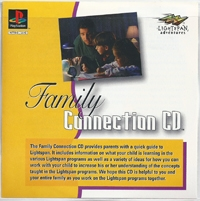
\includegraphics[width=0.5\textwidth]{"./Games/FamilyConnection/Images/FamilyConnectionAGuidetoLightspanCDCover.jpg"}
    \caption{Family Connection: A Guide to Lightspan - CD Cover}
\end{figure}

Family Connection: A Guide to Lightspan was a promotional CD that was produced by The Lightspan Partnership in order to showcase and highlight the importance of integrating technology with education.

The "game" itself, similar to 16 Tales, is split into three sections:

\begin{itemize}
    \item Introducing The Lightspan Partnership
    \item Powerful Learning Programs
    \item Lightspan Adventures
\end{itemize}

Introducing The Lightspan Partnership and Powerful Learning programs are individuals videos on their own.
Lightspan Adventures, on the other hand, is split into three separate videos detailing  the three age groups that Lightspan catered to:

\begin{itemize}
    \item Grades K-2
    \item Grades 3 \& 6
    \item Grades 5 \& 6
\end{itemize}

Each of the Lightspan Adventure series of videos also includes a selection of additional videos highlighting a number of the games which they have on offer.

The combined runtime of all the videos on this CD is just under an hour.

\newpage

\section{List of screenshots:}

\begin{figure}[H]
    \centering
    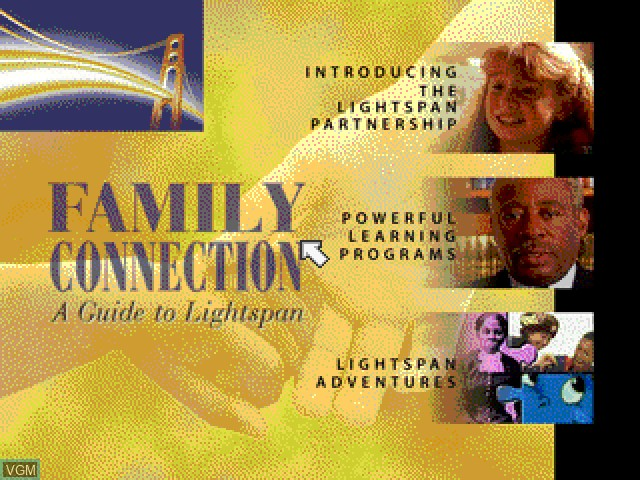
\includegraphics[width=0.5\textwidth]{"./Games/FamilyConnection/Images/FamilyConnectionAGuidetoLightspanMainMenu.jpg"}
    \caption{Screenshot of the main menu}
\end{figure}

\begin{figure}[H]
    \centering
    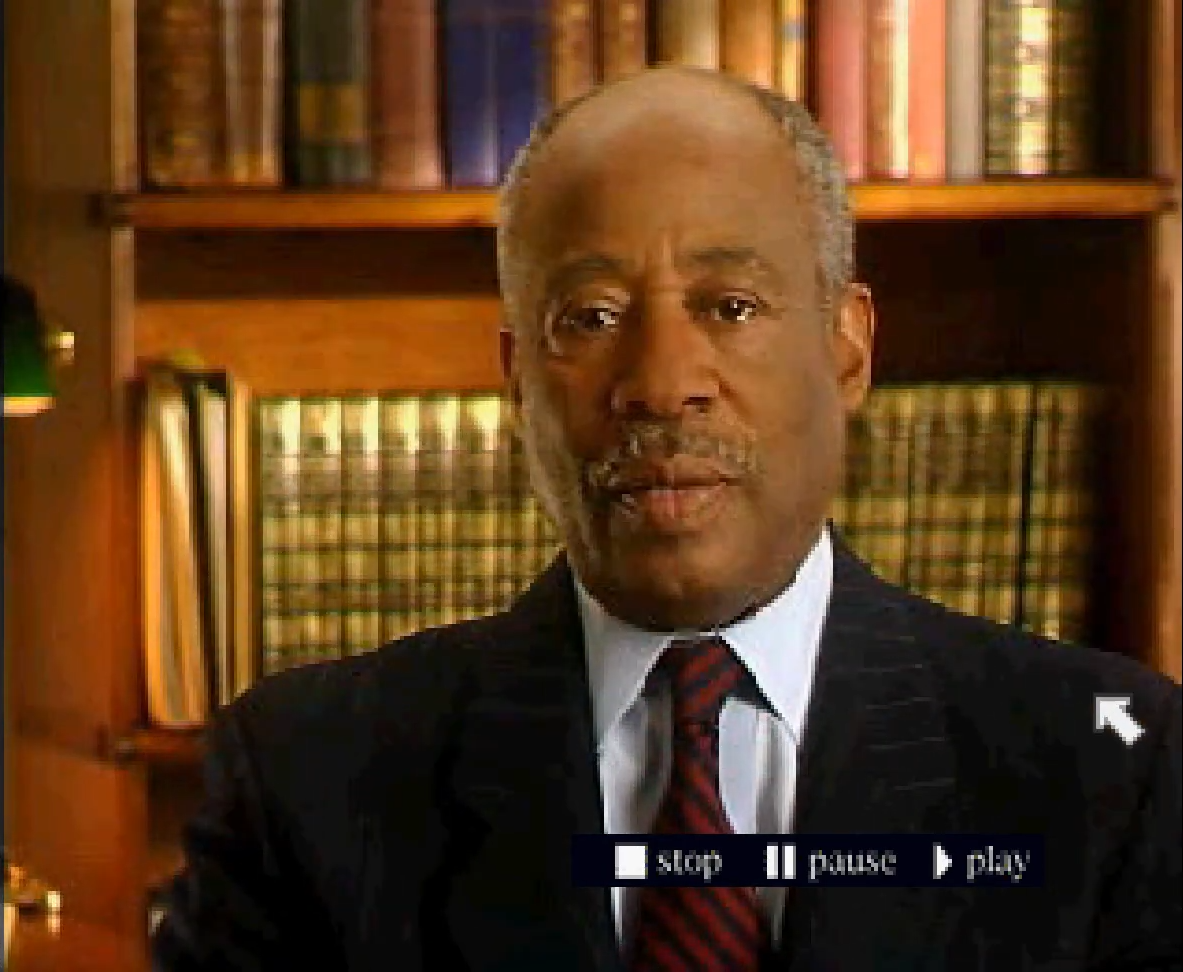
\includegraphics[width=0.5\textwidth]{"./Games/FamilyConnection/Images/FamilyConnectionAGuidetoLightspanScreenshot1.png"}
    \caption{Screenshot taken from the video "Powerful Learning Programs"}
\end{figure}

\begin{figure}[H]
    \centering
    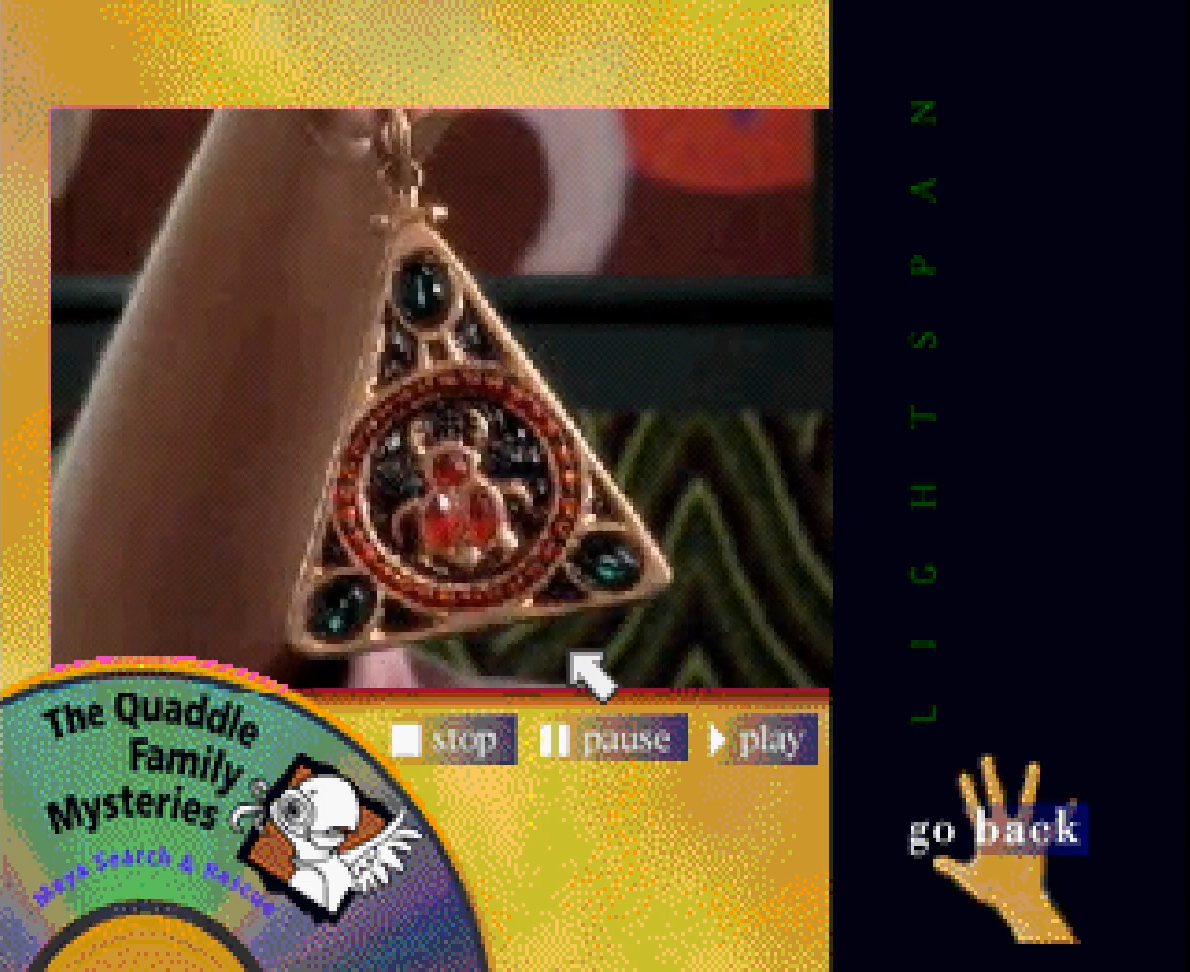
\includegraphics[width=0.5\textwidth]{"./Games/FamilyConnection/Images/FamilyConnectionAGuidetoLightspanScreenshot2.png"}
    \caption{Screenshot from one of the Lightspan Adventures videos}
\end{figure}

\clearpage
\newpage

\section{Main Menu audio transcription}

Welcome to the Family Connection.
We hope this guide to Lightspan will be helpful as you and your family discover new learning opportunities.
Simply click on any of the three pictures to start exploring.

\section{Introducing The Lightspan Partnership audio transcription}

Schools today are surrounded by change - the communities we serve, the kinds of challenges kids face, the demands of the working world have all changed tremendously since I first started teaching.

But one thing will never change - we educators will always have to prepare kids to thrive.
If we're going to keep living up to that responsibility, I think we need to change too.
We have to take the best of what we've always done, reinvent it and make it better. We have to find new tools and new ways of doing things.

The Lightspan Partnership is working with teachers, families, and students to meet today's educational challenges.
We're creating powerful tools that motivate and help children to learn - tools that expand learning in schools and homes, tools that will prepare our children for the challenges of tomorrow.

"Watch what happens when we increase the gravity by just five percent."

"Good, now why do you think that happens?"

There's a natural love of learning in every young child. Our challenge is teachers is to find ways each day to engage that part of them, to nourish it, to focus it on meaningful work so that it keeps growing for a lifetime.

Knowledge and skill grow with practice - learning an idea and then applying it, thinking critically, experimenting, solving problems.
You have to give kids lots of ways to do that.
She can't do it all with a chalkboard.

Kids love great characters and interesting stories.
Who doesn't?
But we need to see more of the time kids spent on entertainment spent on learning.
What if the same people who make the best movies and games would help us educators make things that teach?
Then kids would run home from school and keep on learning whether we told them to or not.
Now that would be a big help.

Teachers and families need to work together to meet the needs of every child.
When parents can see what their children are doing every day, it's easier for them to work together as partners.

"So what did you do in school today?"

"I adjusted my angle by 16 degrees, see, so I would have hit the meteor."

"Oh so look out, look out! So you use geometry to figure out how the rock misses the ship?"

"Yeah!"

"Hey Nick, you did a great job on your history project."

"Thanks, you want to check out Family Activities?"

"Okay."

In sixth grade reading, your child will find more subject material in history and current events.

Powerful educational programming created by some of our finest educators.
Motivating tools designed to challenge and inspire.
An expanded partnership between teachers, students, and families.
This is the Lightspan Partnership.

\section{Powerful Learning Programs audio transcription}

Growing up, I was lucky enough to go to an excellent school with wonderful teachers and to get a terrific education.
And I've devoted most of my life to education as a teacher, counselor, principal, and superintendent.
I was academic vice president at Temple University and was appointed by three presidents - Lyndon Johnson, Jimmy Carter, and Bill Clinton - to national advisory councils on education.

When I went to school, and even when I started teaching, the teacher stood in front of a class while students listened and took notes.
And in most places, that's how teaching is still being done because, for the most part, it works pretty well.
But today there's also an opportunity to use technology to present some of these same ideas and information in ways that I never could with a textbook or a chalkboard - ways that really bring concepts to life and get kids excited about learning.

The Lightspan partnership is working with teachers, families, and students using some of this new technology to develop learning tools that are truly powerful.
The main objective of these programs is to help children learn, so the Lightspan programs start with solid educational content.
They are developed to match the textbooks and other curriculum currently used in your child's classroom, so your child's teacher can easily integrate them into his or her current instruction plans.
And they are developed by expert teachers who have years of successful experience in the classroom.

The focus of these programs is on reading, language arts, and mathematics - the basic skills that we all know are so important for future success.
One of the most important aspects of these programs is that they are flexible and can be tailored to meet the needs of your child.

The Lightspan programs not only teach our children, but they also do so in a way that's motivating, so kids will want to spend time learning because these programs are as much fun and are as exciting as all the other activities that kids enjoy.
And by repeating an activity, they'll master the educational concept, and they'll retain it.
And we all know nothing builds self-confidence and motivation more than success - that sense of accomplishment when we did something that we didn't think we could do.

And for families, Lightspan provides a tremendous opportunity to enhance what children are learning in the classroom by continuing that learning at home.
Parents can see what their child is doing in school, and families can work together with this technology in their own living room whenever they have time.
Lightspan also provides lots of ideas and suggestions for fun, rewarding activities that you can do with your child.

As you work with these programs and see for yourself how your child reacts to them, I am confident that you will see these programs are truly powerful and open up tremendous opportunities for the education of our children.

\section{Lightspan Adventures: Grades K-2 audio transcription}

"My children really love Lightspan.
They love the songs, they love the characters.
They liked interacting with the characters and with the the challenge of it."

"The Lightspan programs teach vocabulary, they teach reading, they teach math in a variety of different ways."

"Blue hat, four-sided head, triangular nose, shiny shoes - that's him."

"And it's very nice because the parent and the child can sit down and work on it together, and they're both involved.
And I think it's just a good way for parents and and children to work together and be working on some of being academic but in a more fun type of way."

"We had an open house, and the first thing the students wanted to show the parents was Lightspan."

"Why don't you tell me what's happening?"

"Okay?"

"And it was so wonderful to see the students showing the parents how they could use it, how they were reading, how they were doing math skills.
And it was wonderful."

\section{Additional Videos}

\subsection{Reading/Language Art: Mars Moose}

\subsubsection{Stay \& Play}

In Stay \& Play, children earn Ranger badges by completing a series of language arts activities.

"Would you guys like to become Rangers?"

Students build on their natural curiosity to explore things in their environment, in this case the inside of the Rangers Clubhouse.
Here students are introduced to basic scientific ideas and concepts that expand their vocabulary and build background knowledge important for future science exploration.
This poster assists students in organizing information and charting their progress.

"Cat. Cat."

In this activity students match audio to corresponding words and pictures.
They learn to associate written text to pictures and strengthen their vocabulary.

"See if you can put the pictures in the correct order."

On the bulletin board, students experiment with ordering events.
They see the pattern in the life cycle of a butterfly, and can extend that knowledge to other patterns in their daily lives.

"You got the life cycle of a butterfly!"

Students also get to experiment with scientific equipment, as in this activity in which students view the moon through a telescope.

Like all Mars Moose Adventures, Stay \& Play invites young children to explore, and helps build a sense of wonder about the natural world.

\subsubsection{Cosmic Quest}

"Wow Cosmo, come back here!"

In Cosmic Quest, students must help Mars Moose get his dog Cosmo down from a tree.
As they assist Mars and the shopkeepers of the town, students learn new words and practice processing and classifying visual information in different settings.

"Try the pet shop!"

This adventure builds students' awareness of environmental text as they read signs and labels around the town.

In the pet store, students identify appropriate animals and move them to specific places.
They use visual and written cues, learning to match words with pictures and developing listening and problem-solving skills.

"Put it to the right of the top fish tank."

They identify words like out, left, bottom, and inside.
In the world of Mars Moose, learning new things is a cause for celebration.
At the pizzeria, children build their background knowledge by expanding their vocabulary with words associated with this type of setting, reinforcing the skills they learned at the pet store.
Students' prior knowledge about recycling is enhanced in this third location, where their vocabulary and experience is extended.
As in the pet store and pizzeria, students practice directional words and learn about sentence structure.
All the while, students are working to help get Cosmo out of the tree.
The celebration in City Park when they succeed is part of the Learning Adventure.

"That's more like it!"

\subsubsection{Walkabout}

"I'm Dr. Diggs!"

In this Walkabout Adventure, students help a paleontologist find bones to reconstruct a dinosaur in a natural history museum.

"Wow, some of his bones are gone!"

"They must be in those three rooms over there."

In each of the rooms of the museum, students develop a variety of language arts skills as they discover facts about the natural world.
In the southwest room, for instance, your child will exercise his or her listening skills, sort a variety of clues, and follow directions to identify specific desert animals.
In the process, they are exposed to information within the text of the story.

"The elf owl hoots."

In the Shipwreck room, your child makes active choices, choosing colors, shapes, or letters.

"F"

In this game, students must remember where letters are located as they match uppercase and lowercase letters.
This activity strengthens their ability to organize and recall new information as it is discovered.
As in every Mars Moose Adventure, success brings an exciting reward and stronger language arts skills.
In the rainforest room, students learn new words and basic sentence structure as they follow directions to identify animals.

"The puma is a type of cat."

Students also make the connection between an animated picture and its real-life image as they view animals in their natural environment.

"Wow, Tyrannosaurus is really cool!"

Through these interactive activities, the Walkabout Adventure shows young children how exciting reading can be.

"It was fun! I can't wait to come back! Bye!"

"Bye."

\subsubsection{Liquid Books}

Fables, poems and riddles come to life in Liquid Books, where children are invited to exercise their imaginations in an engaging environment that exposes them to several distinct types of literature.
The goal in Liquid Books is to become Ranger Reader of the Year by reading all three books.
As they meet this challenge, students practice reading and comprehending written information.
In Under the Pepper Tree, students are introduced to poetry and rhyme structure.
They also learn new vocabulary, including specific animal names and book titles.

"I saw a play with a butterfly and wondered why it fluttered by."

Listening skills are developed in an enjoyable way as students hear the musical quality of the rhyme.
In Who Am I?, students learn about animals found in various habitats.
This setting helps develop a stronger natural science vocabulary.

"Yes, I am an octopus."

By solving riddles about various animals, students develop problem-solving and critical thinking skills.
In African Tales, students evaluate clues and interpret text to identify who is telling the story.

"One day, he stopped and stared. What is this?" he said. "It falls down the mountain and sounds like thunder."

Understanding the author's perspective is one of the key steps on the path to becoming a good reader.
In Liquid Books, students begin to develop an appreciation of literature.
They learn that reading is an exciting experience, full of delightful surprises.

\subsubsection{On Screen Activities - General}

"Look, I'm so glad to see that you're reading!"

Learning with the Lightspan programs can be a rewarding experience for both you and your child.
The on-screen activities provide ideas and suggestions for how you can help to enhance your child's learning as you work on the Lightspan programs together.

"Good job, alright. You want to do another one?"

"Yep."

"Alright. Let's do another one."

\subsubsection{On Screen Activities - Stay \& Play}

The life cycle of a butterfly is presented in Stay and Play.
Talk with your child about the sequence of events in nature.
Ask your child to describe sequential events occurring in his or her life.
For example, baby teeth being replaced with permanent teeth or the process of growing up.

\subsubsection{On Screen Activities - Cosmic Quest}

In Cosmic Quest, children are always eager to fly with Mars Moose through the city.
To help your child learn directional words, encourage him or her to fly Mars to the left and to the right, up and down.

\subsubsection{On Screen Activities - Walkabout}
Distinguishing animal sounds builds a foundation for oral comprehension.
Encourage your child to mimic the animal sounds in the southwest room and then to describe those sounds.

"He sounds like he's hooing!"

Have your child compare his or her description to that provided within the text of the story.

\subsubsection{On Screen Activities - Liquid Books}

Having your child retell a story in his or her own words is a good way to review your child's understanding of the story.

'I'm sorry I had to work late. How are you two doing?'

'Fine."

"Fine."

"Oh, I'm so glad to see that you're reading. This looks like an interesting story. Why don't you tell me what's happening?'

'Okay, let me tell you. A long time ago, an animal went out to see the world.'

'Then he screeched, "I'm the best! I can fly far and fast, and I have colorful feathers, and...'"

'"My bill is long!"'

'Well, I wonder who you are.'

'A bird! He's a bird!'

'Well how do you know that?'

'Because he has feathers, a long bill, and he could fly.'

'Well good, you two figured that one out. Nah, why don't you tell me what happens to this bird.

'Okay, let me start. A one day he stopped and stared. 'What is this?' he said. Then he flapped and flapped, and I forget what comes next.'

'He saw something rolling down the mountain, remember?'

'Look, I have an idea - why don't we look it again and find out what the bird discovers?'

'Okay mom?'

'Oh, here it is. Let's take a look.'

'Turn down the volume so then I could read by myself. One day he stopped and stared. 'What is this?' he said. 'It falls down the hill... no, mountain. It falls down the mountain and sounds like thunder.' Now I know, it's a waterfall!'

'That's right. See the bird finally discovered something that's as great as he is. Now why do you think he was so impressed by that waterfall?'

'Hmm... I don't know, being able to fly would be pretty cool.'

'Yes, but the waterfall is big and powerful and beautiful, and that's great too.'

'I really like listening to that story, but I really really liked hearing you two read.'

\subsubsection{Off Screen Activities - General}

The Educational Concepts introduced in Lightspan's programs can become an exciting part of your child's everyday life.
The off-screen activities provide fun, rewarding activities that you and your child can do together to practice and reinforce the skills learned on lifespan.

\subsubsection{Off Screen Activities - Reading}

The more a child reads, the better.
Set aside some time each day for reading, independently or together.

\subsubsection{Off Screen Activities - Learning directional words}

An enjoyable way to help your child learn directional words is by playing a clue game together.
Take turns creating one or more clues that lead to specific objects in your home.
For example, "I am something that is to the left of the television and on the bookshelf. Do you know what I am?"

\subsubsection{Off Screen Activities - The Wonders of Nature}

Place a potato in water and watch it change over time, or plant seeds outside and watch them grow.
The wonders of nature provide a great opportunity for your child to observe a sequence of events.
Recording the changes in a daily journal also provides practice writing.

\subsubsection{Off Screen Activities - Everyday Activities}

Everyday activities can provide a good way to practice reading skills.
While preparing a meal together, ask your child to identify the letters on a milk carton or to read the back of a cereal box.

\subsubsection{Off Screen Activities - Assisting your child with writing and spelling new words}

As your child is learning to write and spell new words, it may be helpful to draw pictures or simply write down words the way he or she thinks they might be spelled.

"Okay gang, book time!"

"We should have gone to the library today. We don't have any new books to read before bed."

"I know, why don't we make up one of our own stories?"

"New great idea! Carrie, why don't you pick out your favorite color pencil? And hey, buddy, you want to start?"

"There once was a boy who loved to eat peanut butter and pickle sandwiches."

"Yeah, yes, we're off to a good start.
Weird, very weird, but a good start. Alright, whose turn is it?
Mine? Huh, alright, here I go.
Um...
After he had made some amazing Triple Decker peanut butter and pickle sandwiches, he liked to climb under the bed and eat them.
Who's next?"

"I know what I want to say, I'm just not sure how to spell it."

"Oh, honey, it doesn't have to be perfect to start with.
Just spell it the way you think it should be spelled, or you can draw pictures if you want.
"Oh, there's a smile.
Wow, what do you got for us?"

"When he wasn't looking, his little sister liked to sneak big bugs into his sandwiches."

"And so they waved goodbye to the Snowman as the train took off from the station, and they never saw him again.
The end."

"That was a good one!"

"That was a great story.
We should put this on the refrigerator tomorrow morning.
Alright now, let's go to bed, huh?
Yes, sir, it's bedtime. Come on, let's pack it up."

\subsection{Mathematics: The Secret of Googol}

\subsubsection{Tower}

In the Googolheim Tower, many learning situations await students.
With six floors, the tower is an ideal place for students to explore while they learn how geometry is used in everyday situations.

One room definitely worth exploring is the bakery.
Here, students sort dishes according to the geometric shapes and put them inside the correct cubbyhole.
Students look carefully at the number of sides and the relationships among them to classify the shapes.

Also in the bakery, students flip or rotate cookies to match a model.
In this exploration, they see that moving an object does not change its size or shape.

Another of the Tower's rooms students, explore is the stained glass workshop.
In this activity, students complete mirror image patterns on several stained glass window panels.
They learn to visualize reflected images and are introduced to the concept of symmetry.

"On top of my head, the hat is red."

In the toy shop, students use geometric and visual clues to find the correct dolls.
To do so, they must devise a problem-solving strategy to identify and match shapes with their description.

"Great job!"

Designed to appeal to young students' interest in exploring new worlds, the secret of Googol makes learning math an appealing adventure which your child will look forward to again and again.

\subsubsection{Castle}

Wigsley's Castle is the home of Googol's resident eccentric.
Inside the castle, students encountered games and tools that enable them to experience the many uses of geometry in the world.

For example, students use this shape pad tool to build a geometric key that will open the locked castle doors.

Here they learn to visualize, draw, and compare shapes.
This introduces them to the concept of congruence - figures of the same shape and size.

In this three-dimensional environment, students experience math concepts in compelling ways that are difficult to show using textbooks alone.
The power of multimedia allows students to see solid objects unfold in front of them, as with this cube.

In this activity, students shoot darts to land inside, outside, or on one of the specified shapes.
In the process, they practice identifying shapes and learn the meaning of words that indicate position.

Many of the games have a help button which provides assistance when needed.

In this game, students must remember the location of tiles that match other tiles.
They gain practice defining shapes and matching shapes to their descriptions.

"Okay Cali, make a triangle!"

The Secret of Googol offers many opportunities for students to be active problem solvers, and provides the practice necessary to build a strong foundation for future success in mathematics.

\subsubsection{Ocean}

Within the fanciful world of Googol, there's a collection of fast-paced games in the ocean designed to provide students with the practice they need to master basic math concepts.
Students explore the ocean environment from inside the submarine by peering through these windows.

In this fast action game, students refuel the submarine by identifying geometric shapes.
This provides plenty of practice and gives immediate feedback, a powerful tool for student motivation.
The reward animation is designed to provide encouragement for student effort.

"What has 1 five-sided shape and 2 triangles?"

Looking through another window, students try to feed a squid by identifying shapes and combinations of shapes in a natural setting.
Using geometric clues, students search the caves for the sea creature that matches the voiced and written description.
This exploratory activity allows time to develop problem-solving strategies and helps strengthen memory skills as students keep track of which creature was in which cave.

Students are motivated to learn math skills when they find that math is an enjoyable problem-solving activity with its own reward.
That's life in Googol.

\subsubsection{Sub}

Inside the submarine, students use their mathematical problem-solving skills to solve puzzles and recognize patterns.
As a first step, they must gain entry.

"We need to open the hatch."

To unlock the submarine hatch, students must complete the geometric pattern.
In doing so, they gain practice recognizing and completing geometric patterns.

"Wow! the door's opening!"

Once inside the sub, students can experiment with the control panel instruments.
In this game, students solve a series of tangram puzzles.
They learn to investigate and predict the results of combining basic geometric shapes to form a more complex shape.

Students' efforts are rewarded with positive feedback that relates the geometric creations to the natural world.

To open the submarine's periscope, students must remember the pattern of geometric shapes shown earlier.
Once students have completed all the activities\dots

"Ready to cruise!"

\dots the sub is ready to cruise.
It's one of the exciting learning activities in the world of Googol!

\subsubsection{On Screen Activities - Match shapes to written descriptions}

In this activity, children match shapes to written descriptions.
One way to help your child find matches in a game like this is to make a chart.
Have your child write down what is revealed behind each tile to remember where the clues are located.

\subsubsection{On Screen Activities - Reflected Images}

One way to help your child see a shape's reflected image and to gain a better understanding of symmetry is by using an ordinary mirror.
Compare the image in the mirror to the image on the screen.
You may want to point out that the images are opposites.

\subsubsection{On Screen Activities - Recognise the pattern of shapes}

To help your child recognize and complete the pattern of shapes, try saying the name of each shape together out loud.

"Square, square. Triangle, triangle."

Another way to help identify the pattern is by calling out the number of sides of each shape.

"Four, four. Three, three."

\subsubsection{On Screen Activities - Explore Underwater Caves}

In this activity, children search the underwater caves to identify shapes and combinations of shapes that match the written descriptions.
To help keep track of which creature lives in which cave, you and your child can create a map.
Have your child draw a picture or write a description of what he or she finds in each cave.

\subsubsection{On Screen Activities - Repeating}

Drawing a picture, rewriting, or verbally repeating are all ways to recall information.
Helping your child to identify the most effective method for him or her can help develop important study skills.

"Well, let's see. And we got a rectangular fan, shiny shoes, a triangular nose, a blue hat.
You know, this is a pretty good riddle.
But you know what, all these clues are a little much for me to try to keep in my head, so what I'm going to do is I'm going to draw a picture of what the clown's going to look like."

"I have another idea."

"Hmm?"

"I'm going to keep saying the clues, that's how I'll remember them.
Rectangular fan, shiny shoes, triangular nose, blue head."

"Well, that'll work too.
You know, we all have different little tricks to help us learn, huh?
You know, some people need to look at things so they can see what's happening.
Others need to draw a picture or write things down.
But if you can remember these things by repeating them, then that's great too."

"Okay, here we go.
It's not the clown on the right, because he has a square nose, and the one in the middle has a green head.

"Mmm, hmm, so it's not either of those two, and it can't be that guy because his fan is the wrong shape, huh?
Well, we are narrowing it down."

"Ther's only two left, and it's this one.
Blue hat, four-sided head, triangular nose, shiny shoes. That's him."

"You solved the riddle!
Good job!
Alright, you want to do another one?"

"Yep."

"Alright, let's do another one."

\subsubsection{Off Screen Activities - Symmetry birthday card}

The next time a birthday comes up, why not help your child make a symmetry birthday card?
First, fold a piece of paper in half.
Then draw and cut out one side of a butterfly.
Next, open the card and place a few drops of food coloring on one side of the card only.
Fold the paper again, pressing both sides of the butterfly together.
Then unfold it to see the symmetrical design you've created.

\subsubsection{Off Screen Activities - Learning through everyday activities}

Everyday activities like putting away dishes and utensils of various shapes, colors, and sizes provide an ideal opportunity for your child to practice classifying and sorting.

\subsubsection{Off Screen Activities - Identify geometric shapes of road signs}

The next time you and your child are riding in a car, have your child identify the geometric shapes of road signs.
For example, pointing out the triangular shape of a yield sign.
Your child can also draw and chart the road signs he or she sees during a variety of outings.

\subsubsection{Off Screen Activities - Art and Geometry}

Art and geometry have a lot in common.
Ask your child to create a masterpiece by using only geometric shapes.

\subsubsection{Off Screen Activities - Preparing a picnic}

Everyday activities such as preparing a picnic can become an opportunity to apply geometry outside the classroom.

"Look, I cut my sandwich into triangles, and now it's a butterfly!"

"Butterfly? Well, don't let it fly away.
You sure know your shapes Mehita.
You like learning geometry, don't you?"

"Yes, I see shapes everywhere."

"Hey, this is a rectangle, right?"
Now it's a square."

"Oh yeah, but what are these?"

"Anna, those are rectangles again, just like these halves of my sandwich."

"That's right, Mikita.
Oh, what about this cheese?
What shape is this?"

"That's a triangle.
You know what?
It's three-dimensional."

"Oh, you're right."

"This orange is a sphere."

"It sure is.
You know, you're all doing so well learning your geometry.
But now we're going to do something that's going to help us with our fractions too."
I have a perfectly round pumpkin pie that we're going to divide up into five equal pieces.
Now, how are we gonna do it?"

"I know, that's easy!"

"Let's have some right now!"

"That sounds good. Pass the knife."

\section{Lightspan Adventures: Grades 3 \& 4 audio transcription}

"Lightspan corresponds perfectly with the curriculum that we're using today.
It goes along with all of the books that we're using, all of the programs that provide us with information on prefixes and suffixes - everything.
Lightspan helps to bridge the connection between the home and the teacher and the child"

"I think Lightspan has encouraged parents and teachers to work together because there's a common thread now, both at school and at home."

"Let me show you how. You take the highlighted word..."

"The kids can't wait to get on Lightspan, and sometimes I have to hold them back."

"I think Lightspan has been a giant step, bringing technology into the classrooms."

\subsection{Reading/Language Arts: Mona \& Moki}

"Everything's a possibility."

"Camera."

"Books and documentaries."

Mona and Loki's world is a place of contrast, including many in the English language.
In this adventure, your child works with synonyms, antonyms, prefixes, and suffixes.
Students also solve riddles and develop critical thinking skills.

-------------------Up to here----------------

43:48

\subsubsection{On Screen Activities - Scrambled Letters}

To help your child form words from scrambled letters, encourage him or her to experiment with the order of the letters.
Many times, the hidden word is not obvious, and experimenting is a good strategy for solving this type of puzzle.

\subsubsection{On Screen Activities - Visualising Words}

Sometimes visualizing a word will help your child understand how a suffix affects meaning.

"Baker. Bakery. Baked"

\subsubsection{On Screen Activities - The Meaning of Prefixes}

Before playing the prefix game in Euripides' Eatery, help your child understand the meaning of prefixes such as "post", "re", or "auto" by playing a guessing game.

"Would you like a post-dinner snack tonight?"

"Post-dinner? Desert. 'Post' means 'after'."

\subsubsection{On Screen Activities - Using the Process of Elimination}

Learning to use the process of elimination to determine a correct answer is a valuable problem-solving strategy.
Another problem-solving method is to think of your own answer before looking at those provided.

"Oh man, I made a mistake and I lost my points."

"You did?
Ah, well we can't win them all, but let's give it another try though.
I'm sure we'll do better next time."

"Okay dad, let me show you.
You take the highlighted word and match it to the word on the list that means the same thing.
They're synonyms."

"Hey, here's an idea.
How about if we make up our own list of synonyms, you know, answers that make sense to us, and then we'll see how many of our words match those on that list?"

"Okay."

"Okay, we'll just cover up these words and make up a few of our own.
Go ahead and read the sentence."

"The library will keep the book for Sarah."

"Okay, now what are some words that have the same meaning as 'keep'?"

"Uh, hold? Save?"

"That's right.
Let's see, now are those words on the list?"

"No, but maybe there's one that's close."

"Hmm, yeah."

"Hey, I've got an idea!
How about if we cover up the words we know don't mean the same thing as 'keep'?"

"That's good thinking.
That way, we narrow it down, huh?
I've got just the thing to help us out too."
Here you go.
How about the word 'thief'?

"The library will thief the book for Sarah.
I don't think that fits."

"No, me either, so we'll go ahead and cover that up."

"This is a good idea dad. We'll cover up all the words we know are wrong, and then we'll end up with the word that matches."

"Mmm hmm, that's right. Maybe we'll get to keep all our points, huh?
Better yet, we'll learn lots of synonyms, right?"

"That's correct. Correct right. Hey, those are synonyms."

"You're right again."

\subsubsection{Off Screen Activities - Synonyms and Antonyms}

To help your child practice using prefixes and suffixes, pick a prefix or suffix to play with for several days.
Each day, create a new word using your prefix or suffix and practice using the word in sentences.
For example, with the prefix "auto", you can create words such as automobile, autograph, or autobiography.

\subsubsection{Off Screen Activities - Create a Story for your Child}

Create a story with your child that includes as many descriptive words as possible.
Having your child then replace the descriptive words with their antonyms, opposites, can lead to unexpected changes in the story and an evening of family fun.

\subsubsection{Off Screen Activities - Word Scramble Fun with Signs}

Everyday signs take on new meaning when you play with their letters.
Practice critical thinking skills with your child by scrambling the letters in signs to create new words.

\subsubsection{Off Screen Activities - Create Riddles}

Your child can add intrigue to an ordinary dinner and develop his or her critical thinking skills at the same time.
Have your child create a mystery menu with riddles that describe the various foods.

"I'm thin as a pin and I'm ready to spin, what am I?"

Others at the table must solve the riddles before they are allowed to eat.

\subsubsection{Off Screen Activities - Magazine and Newspaper Cutting}

Have fun with prefixes, suffixes, and all kinds of new vocabulary by cutting out words from magazines or newspapers and reordering them to create an original story with your child.

\subsubsection{Off Screen Activities - }

"So do you have a lot of homework today?"

"Not too bad.
We're supposed to find antonyms around the house."

"Ants? I sure hope there aren't any ants crawling around our kitchen."

"Mom.
You know, antonyms, words that mean the opposite of each other?"

"Right? We could probably find a few of those right now.
Let's see...
The sugar in my tea is sweet and the lemon is sour.
Your turn."

"Hmm...
I know!
Your tea is hot and my juice is cold.
Now it's your turn."

"You got it!
Hey, I have a great idea for a good antonym game we can play when your friends come over."

"Cool!"

"Here's how the game works: I'll pick a word from the dictionary, and each team will have exactly one minute to write down as many antonyms as you can think of for that word.
Then, we'll go over them.
Each team will earn five points for each correct antonym.
If we're not sure what the word means, we'll look it up in the dictionary.
Okay?"

"Okay, got it!"

"And the first word is 'sad'."

"On your mark... Get set... Go!"

"Playing a simple word game with family and friends is a great way to learn synonyms or antonyms."

\subsection{Mathematics: Quaddle Family Mysteries}

"The Quaddle Family Mysteries" is an interactive mathematics program that challenges students to use their problem-solving skills to find the answers to some puzzling mathematical mysteries.
In the case of the scarce scarab, students explores and solve mathematical problems related to measurement in order to find the missing scarab earring.

"And now, there's only one, and this shiny button."

Students will have to use their critical thinking skills to solve this case.
No matter where they roam in the Quaddle Museum, they will find that PK Macaw is always available to explain how to complete the activities.
In the Quaddle Kitchen, students can choose to bake cookies, muffins, or cakes.
Following recipes from the cookbook, students find that mathematics, in this case, the concepts of capacity and fractions, is relevant to everyday situations.
Help in understanding mathematical concepts is always readily available within the games.

"One-third cup plus one-third cup equals two-thirds cup.
Plus another third cup equals one cup."

Results are surprising, which makes students want to play the games again and again.
As the plot thickens, students are compelled to continue investigating.
Back at the museum's Lobby, students weigh letters to determine if the missing earring is in one of them.
Here, students gain valuable experience reading charts, interpreting data, and calculating the correct amount of postage based on the weight of a letter and its destination.
Once again, they learn that understanding measurements is useful in everyday situations.

"Can I help too?"

Students will have other opportunities to develop their math skills and solve mysteries in the Quaddles Garden, Family Room, and Parlor - all part of the Quaddle Family Mysteries' first adventure.

"You could even start right here in this room."

\section{Lightspan Adventures: Grades 5 \& 6 audio transcription}

"My students really enjoy Lightspan.
It's very appealing to them.
They like the graphics, they like the storyline.
It's very age appropriate for them.
They choose to do it when they have free time, spare time."

"When the Lightspan program stratus goes into the home, with parents and students working together, I see that there's going to be a lot of communication happening between parent and child, as well as problem solving."

"So what did you do in school today?"

"I adjusted my angle by 60°."

"The Lightspan concept of parents and families and teachers and students all working together is a very, very important one."

"You want to check out Family Activities?"

"Okay."

"If students are using the Lightspan program at home with their parents, they'll be actually reading more.
They're also learning about characters in history, they're problem solving, they're learning vocabulary.
So this can only benefit their education."

\subsection{Mathematics: Timeless Math}

"The Mayans were obsessed with time measurements.
They developed a complex calendar which reached into the past and forward into the future."

In the first adventure of Timeless Math, Todd and Maria are transported back to the ancient world of the Maya where they must solve a number of mathematical problems to return home.

In the Search and Rescue segment of the Maya adventure, students practice fundamental skills pertaining to fractions, decimals, and percentages.

In the Jewel Pick game, students passes through the tunnels of a Maya pyramid by selecting the correct number of jewels represented as part of the whole.
When students make incorrect choices, they are encouraged to try again.

In the Rope Climb Challenge, students cross a maze of ropes by moving to the correct positions which correspond to fractions, decimals, and percentages in the context of a number line.
Once across, students obtain immediate feedback on their performance and have the opportunity to replay the game and improve their scores.

At the Falling Floor, students match fractions, decimals, or percentages to their equivalent amounts represented by colored areas on the floor tiles.
At higher levels, problems are more challenging.
When students are having a difficult time solving problems, they have immediate access to instructional help.

"There's no time to explain!
We got to go!"

Students ultimately accomplish their mission by completing numerous activities and returning to the present day.

When students use Timeless Math, they are building solid foundations in mathematics and having fun along the way.

\subsection{Reading/Language Arts: str.at.\reflectbox{e}s}

"This is str.at.\reflectbox{e}s"

str.at.\reflectbox{e}s is a dynamic game in which your child will develop reading comprehension and vocabulary skills in the context of a time travel adventure.

Through a chance occurrence at Ms. Stafford's house, four students are sent into the 1800s and early 1900s

"I'm on a train in a place called Mud Run."

Your child assumes the character of one of these students as he or she reads about people, then plays vocabulary and reading strategy games to return to Ms. Stafford's home.